\subsection{Performance Requirements}
\begin{itemize}
	
\end{itemize}
\subsection{Design Constraints}
\begin{enumerate}
	
\end{enumerate}
\subsection{Software System Attributes}



\subsection{Class diagram}
 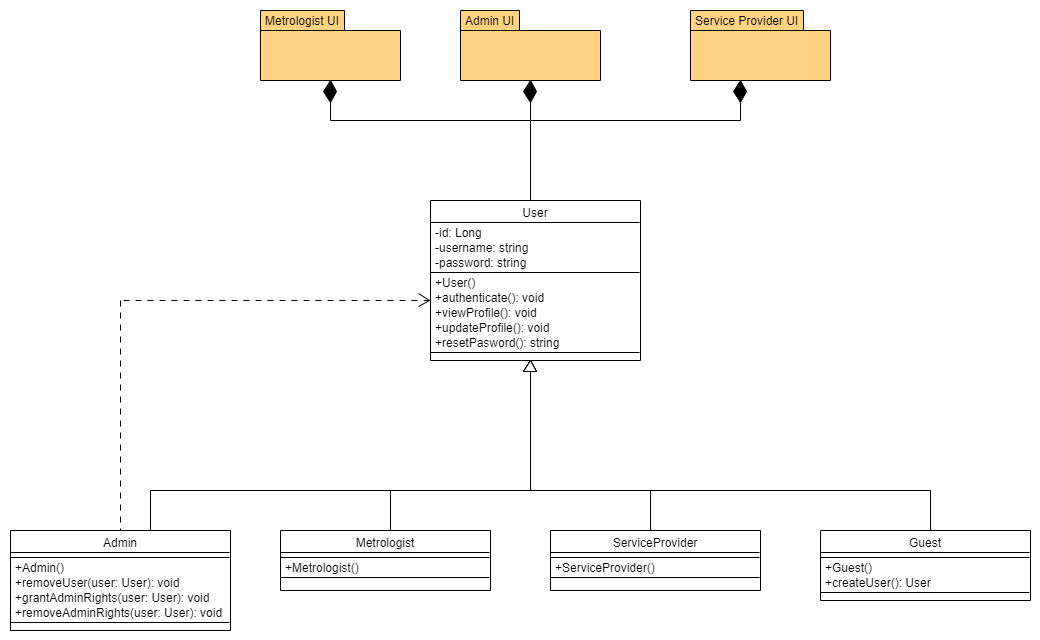
\includegraphics[width=12cm,height=26cm,keepaspectratio]{users_unit/Images/users class diagram.png}
	\begin{center}
	    \small{Figure 6: Class diagram for Users}
    \end{center}
\paragraph{Design Patterns Used}
	
	
		
\subsection{Activity diagram}
    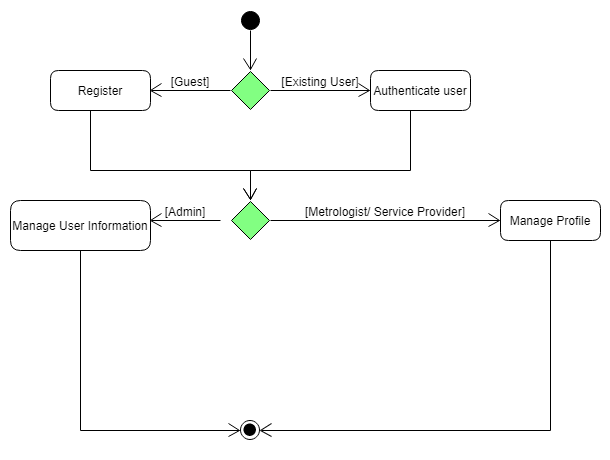
\includegraphics[width=12cm,height=26cm,keepaspectratio]{users_unit/Images/users activity diagram.png}
	\begin{center}
	    \small{Figure 7: Activity diagram for Users}
    \end{center}


\subsection{Sequence diagram}
    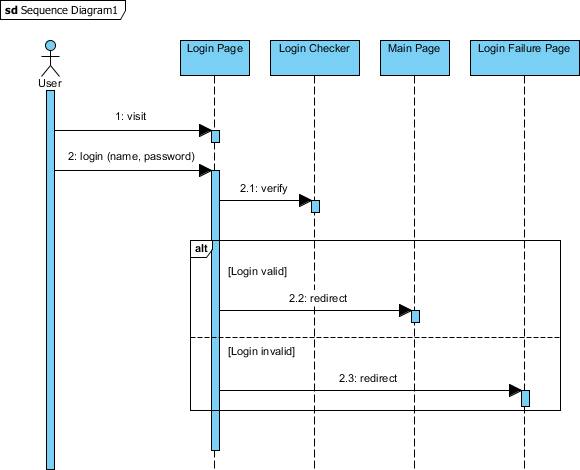
\includegraphics[width=12cm,height=26cm,keepaspectratio]{users_unit/Images/users sequence diagram.png}
	\begin{center}
	    \small{Figure 8: Sequence diagram for Users }
    \end{center}

\subsection{State diagram}
    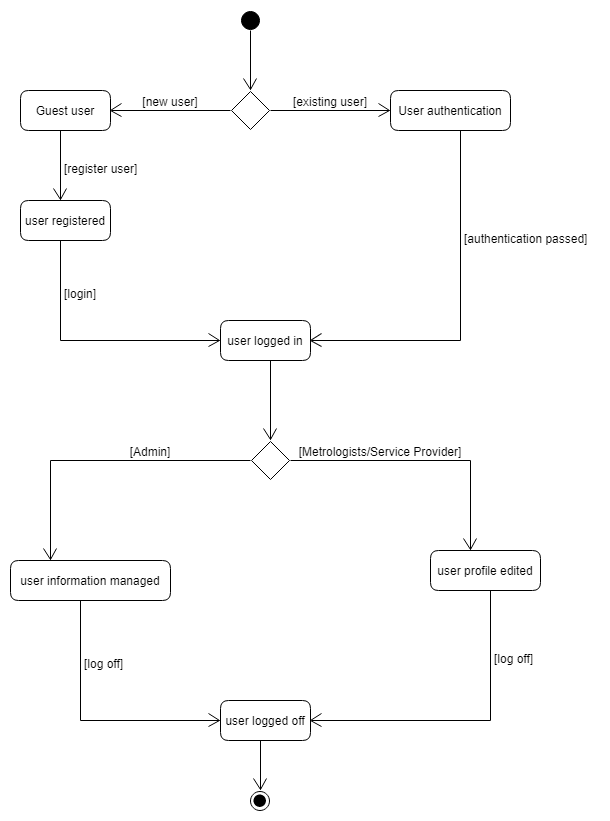
\includegraphics[width=12cm,height=26cm,keepaspectratio]{users_unit/Images/users state diagram.png}
	\begin{center}
	    \small{Figure 9: State diagram for Users}
    \end{center}




\subsection{Use Case diagram}
   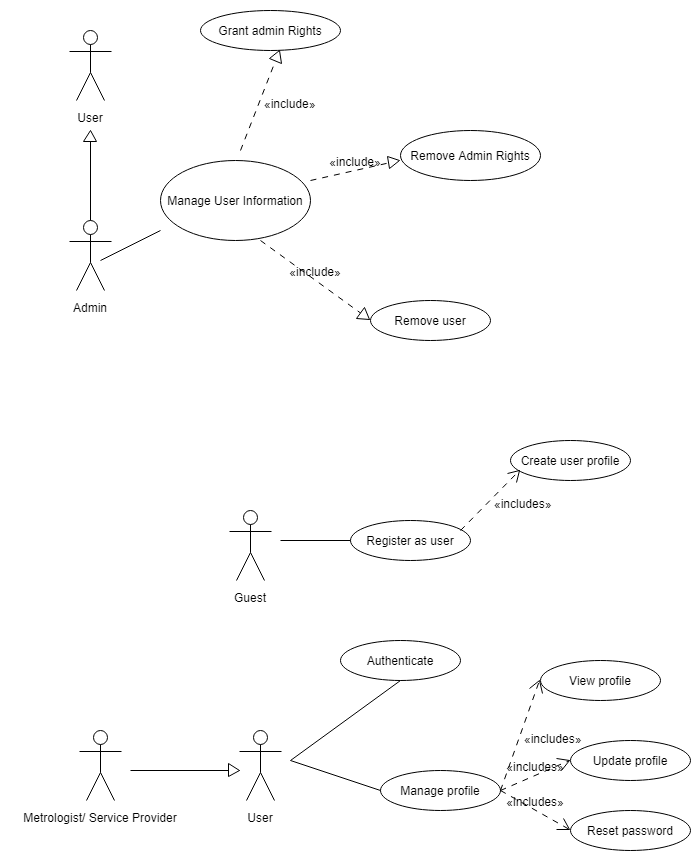
\includegraphics[width=12cm,height=26cm,keepaspectratio]{users_unit/Images/users use case diagram.png}
    \begin{center}
    	\small{Figure 10: Use case diagram for Users}
    \end{center}